%!TeX encoding = utf8
%!TEX TS-program = xelatex
\documentclass{standalone}

%\usepackage{ctex} %%需要显示中文时用

\usepackage{tikz}
\usetikzlibrary{shapes,positioning}

%%定义流程图的各种符号
\tikzstyle{inout}=[trapezium, trapezium left angle=60, trapezium right angle=120, draw] %%输入输出框
\tikzstyle{end}=[rectangle, rounded corners, draw]   %%教材上的起止框
\tikzstyle{endn}=[rounded rectangle, draw]   %%新版的起止框
\tikzstyle{exec}=[rectangle, draw]    %%执行框 execute
\tikzstyle{decide}=[kite, kite vertex angles=120, draw]   %%判断框

\begin{document}

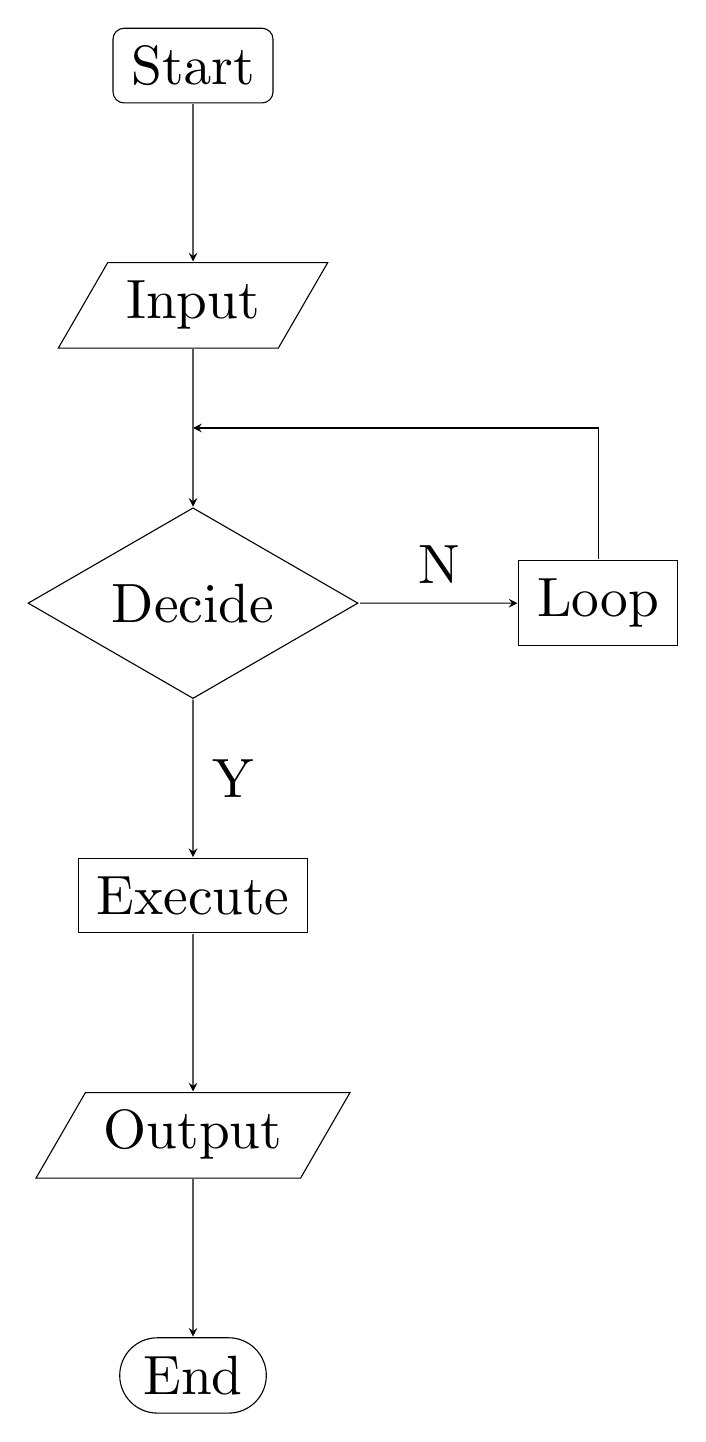
\begin{tikzpicture}[-stealth,scale=2,transform shape]

\node[end] (s) at (0,0) {Start};
\node[inout] (i) [below=of s] {Input};
\node[decide] (d) [below=of i] {Decide};
\node[exec] (l) [right = of d] {Loop};
\node[exec] (c) [below=of d] {Execute};
\node[inout] (o) [below=of c] {Output};
\node[endn] (e) [below=of o] {End};

\draw (s) -- (i);
\draw (i) -- coordinate (le) (d); %%给循环回来的箭头给终点 (le)
\draw (d) -- node [right] {Y} (c);
\draw (d) -- node [above] {N} (l);
\draw (l) |- (le);
\draw (c) -- (o);
\draw (o) -- (e);

\end{tikzpicture}



\end{document}